\PassOptionsToPackage{svgnames,dvipsnames,svgnames}{xcolor}

\documentclass[nonacm]{acmart}
\settopmatter{printfolios=true,printccs=false,printacmref=false}

%% Conference information
%% Supplied to authors by publisher for camera-ready submission;
%% use defaults for review submission.
%% ?

%% Copyright information
%% Supplied to authors (based on authors' rights management selection;
%% see authors.acm.org) by publisher for camera-ready submission;
%% use 'none' for review submission.
\setcopyright{none}
%\setcopyright{acmcopyright}
%\setcopyright{acmlicensed}
%\setcopyright{rightsretained}
%\copyrightyear{2019}           %% If different from \acmYear

%% Bibliography style
\bibliographystyle{ACM-Reference-Format}
%% Citation style
%\citestyle{acmauthoryear}  %% For author/year citations
%\citestyle{acmnumeric}     %% For numeric citations
%\setcitestyle{nosort}      %% With 'acmnumeric', to disable automatic
                            %% sorting of references within a single citation;
                            %% e.g., \cite{Smith99,Carpenter05,Baker12}
                            %% rendered as [14,5,2] rather than [2,5,14].
%\setcitesyle{nocompress}   %% With 'acmnumeric', to disable automatic
                            %% compression of sequential references within a
                            %% single citation;
                            %% e.g., \cite{Baker12,Baker14,Baker16}
                            %% rendered as [2,3,4] rather than [2-4].


%% Some recommended packages.
\usepackage{booktabs}   %% For formal tables:
                        %% http://ctan.org/pkg/booktabs
\usepackage{subcaption} %% For complex figures with subfigures/subcaptions
                        %% http://ctan.org/pkg/subcaption

\usepackage{microtype}
\usepackage{mdframed}
\usepackage{colortab}
\usepackage{mathpartir}
\usepackage{enumitem}
\usepackage{bbm}
\usepackage{stmaryrd}
\usepackage{mathtools}
\usepackage{leftidx}
\usepackage{todonotes}
\usepackage{xspace}
\usepackage{wrapfig}
\usepackage{float}

\usepackage{listings}%
\lstloadlanguages{ML}
\lstset{tabsize=2, 
basicstyle=\footnotesize\ttfamily, 
% keywordstyle=\sffamily,
commentstyle=\itshape\ttfamily\color{gray}, 
stringstyle=\ttfamily\color{purple},
mathescape=false,escapechar=\#,
numbers=left, numberstyle=\scriptsize\color{gray}\ttfamily, language=ML, showspaces=false,showstringspaces=false,xleftmargin=10pt, 
morekeywords={string, float, int},
classoffset=0,belowskip=\smallskipamount, aboveskip=\smallskipamount,
moredelim=**[is][\color{red}]{SSTR}{ESTR}
}
\newcommand{\li}[1]{\lstinline[basicstyle=\ttfamily\fontsize{9pt}{1em}\selectfont]{#1}}
\newcommand{\lismall}[1]{\lstinline[basicstyle=\ttfamily\fontsize{9pt}{1em}\selectfont]{#1}}
\newcommand{\dd}{\emph{delta dict}}
\newcommand{\mapP}{\{0 \rightarrow \text{"a"}, 1 \rightarrow \text{"b"}, 3 \rightarrow \text{"c"}, 6 \rightarrow \text{"d"}, 10 \rightarrow \text{"e"}\}}

%% Joshua Dunfield macros
\def\OPTIONConf{1}%
\usepackage{joshuadunfield}

%% Can remove this eventually
\usepackage{blindtext}

\usepackage{enumitem}

% \newtheorem{theorem}{Theorem}[chapter]
% \newtheorem{lemma}[theorem]{Lemma}
% \newtheorem{corollary}[theorem]{Corollary}
% \newtheorem{definition}[theorem]{Definition}
% \newtheorem{assumption}[theorem]{Assumption}
% \newtheorem{condition}[theorem]{Condition}

\newtheoremstyle{slplain}% name
  {.15\baselineskip\@plus.1\baselineskip\@minus.1\baselineskip}% Space above
  {.15\baselineskip\@plus.1\baselineskip\@minus.1\baselineskip}% Space below
  {\slshape}% Body font
  {\parindent}%Indent amount (empty = no indent, \parindent = para indent)
  {\bfseries}%  Thm head font
  {.}%       Punctuation after thm head
  { }%      Space after thm head: " " = normal interword space;
        %       \newline = linebreak
  {}%       Thm head spec
\theoremstyle{slplain}
\newtheorem{thm}{Theorem}  % Numbered with the equation counter
\numberwithin{thm}{section}
\newtheorem{defn}[thm]{Definition}
\newtheorem{lem}[thm]{Lemma}
\newtheorem{prop}[thm]{Proposition}
% \newtheorem{cor}[section]{Corollary}     
% \newtheorem{lem}[section]{Lemma}         
% \newtheorem{prop}[section]{Proposition}  

% \setlength{\abovedisplayskip}{0pt}
% \setlength{\belowdisplayskip}{0pt}
% \setlength{\abovedisplayshortskip}{0pt}
% \setlength{\belowdisplayshortskip}{0pt}

\fancyfoot{} % suppresses the footer (also need \thispagestyle{empty} after \maketitle below)

% !TEX root = main.tex

\newcommand{\mynote}[3]{\textcolor{#3}{\textsf{{#2}}}}
\newcommand{\rkc}[1]{\mynote{rkc}{#1}{blue}}
\newcommand{\nick}[1]{\mynote{cy}{#1}{purple}}

\newcommand{\cvert}{{\,{\vert}\,}}

%% https://tex.stackexchange.com/questions/9796/how-to-add-todo-notes
\newcommand{\rkcTodo}[1]{\todo[linecolor=blue,backgroundcolor=blue!25,bordercolor=blue]{#1}}

\newcommand{\mattTodo}[1]{\todo[linecolor=green,backgroundcolor=green!2,bordercolor=green]{\tiny\textit{#1}}}
\newcommand{\mattOmit}[1]{\colorbox{yellow}{(Matt omitted stuff here)}}

\def\parahead#1{\paragraph{\textbf{#1.}}}
%% \def\paraheadNoDot#1{\paragraph{{\textbf{#1}}}}
\def\subparahead#1{\paragraph{\textit{#1.}}}
%% \def\paraheadindent#1{\paragraph{}\textit{#1.}}
%% \def\paraheadindentnodot#1{\paragraph{}\textit{#1}}

\newcommand{\ie}{i.e.}
\newcommand{\eg}{e.g.}
% \newcommand{\etc}{{\emph{etc.}}}
% \newcommand{\cf}{{\emph{cf.}}}
% \newcommand{\etal}{{\emph{et al.}}}

%% \newcommand{\hazel}{\ensuremath{\textsc{Hazel}}}
%% \newcommand{\sns}{\ensuremath{\textsc{Sketch-n-Sketch}}}
%% \newcommand{\deuce}{\ensuremath{\textsc{Deuce}}}
\newcommand{\Elm}{\ensuremath{\textsf{Elm}}}
\newcommand{\sns}{\ensuremath{\textrm{Sketch-n-Sketch}}}
\newcommand{\deuce}{\ensuremath{\textrm{Deuce}}}

\newcommand{\sectionDescription}[1]{\section{#1}}
\newcommand{\subsectionDescription}[1]{\subsection{#1}}
\newcommand{\subsubsectionDescription}[1]{\subsubsection{#1}}
%% \newcommand{\subsectionDescription}[1]{\subsection*{#1}}
\newcommand{\suppMaterials}{the Supplementary Materials}

\newcommand{\defeq}{\overset{\textrm{def}}{=}}

\newcommand{\eap}{action suggestion panel\xspace}
\newcommand{\Eap}{Action suggestion panel\xspace}

\newcommand{\myfootnote}[1]{\footnote{ #1}}

\def\sectionautorefname{Section}
\def\subsectionautorefname{Section}
\def\subsubsectionautorefname{Section}

\newcommand{\code}[1]{\lstinline{#1}}
\newcommand{\str}[1]
  {``#1''}

% Make italic?
%\newcommand{\Property}[1]{\emph{#1}}
\newcommand{\Property}[1]{\textrm{#1}}

% Calling out Cyrus's favorite verb, 'to be' ;)
\newcommand{\IS}{\colorbox{red}{is}\xspace}

\newcommand{\codeSize}
  %% {\footnotesize}
  {\small}

%\newcommand{\JoinTypes}[2]{\textsf{join}~~#1~~#2}
\newcommand{\JoinTypes}[2]{\textsf{join}(#1,#2)}

%% \newtheorem{theorem}{Theorem}[section] % 2.1, 2.2, etc.
\newtheorem{theorem}{Theorem}             % 1, 2, etc.
\newtheorem{remark}[theorem]{Remark}

%%%%%%%%%%%%%%%%%%%%%%%%%%%%%%%%%%%%%%%%%%%%%%%%%%%%%%%%%%%%%%%%%%%%%%%%%%%%%%%%
%% Spacing

\newcommand{\sep}{\hspace{0.06in}}
\newcommand{\sepPremise}{\hspace{0.20in}}
\newcommand{\hsepRule}{\hspace{0.20in}}
\newcommand{\vsepRuleHeight}{0.08in}
\newcommand{\vsepRule}{\vspace{\vsepRuleHeight}}
\newcommand{\miniSepOne}{\hspace{0.01in}}
\newcommand{\miniSepTwo}{\hspace{0.02in}}
\newcommand{\miniSepThree}{\hspace{0.03in}}
\newcommand{\miniSepFour}{\hspace{0.04in}}
\newcommand{\miniSepFive}{\hspace{0.05in}}
\newcommand{\breakAndIndent}
  {\mbox{}

   %% \hspace{0.15in}
   \hspace{0.00in}
  }

\newcommand{\justIndent}
  %% {\hspace{0.15in}
  {\hspace{0.00in}
  }

%%%%%%%%%%%%%%%%%%%%%%%%%%%%%%%%%%%%%%%%%%%%%%%%%%%%%%%%%%%%%%%%%%%%%%%%%%%%%%%%

% \lstset{
% %mathescape=true,basicstyle=\fontsize{8}{9}\ttfamily,
% literate={=>}{$\Rightarrow$}2
%          {<=}{$\leq$}2
%          {->}{${\rightarrow}$}1
%          {\\\\=}{\color{red}{$\lambda$}}2
%          {\\\\}{$\lambda$}2
%          {**}{$\times$}2
%          {*.}{${\color{blue}{\texttt{*.}}}$}2
%          {+.}{${\color{blue}{\texttt{+.}}}$}2
%          {<}{${\color{green}{\lhd}}$}1
%          {>?}{${\color{green}{\rhd}}$?}2
%          {<<}{${\color{green}{\blacktriangleleft}}$}1
%          {>>?}{${\color{green}{\blacktriangleright}}$?}2
%          {\{}{${\color{blue}{\{}}$}1
%          {\}}{${\color{blue}{\}}}$}1
%          {[}{${\color{purple}{[}}$}1
%          {]}{${\color{purple}{]}}$}1
%          {(}{${\color{darkgray}{\texttt{(}}}$}1
%          {)}{${\color{darkgray}{\texttt{)}}}$}1
%          {]]}{${\color{gray}{\big(}}$}1
%          {]]}{${\color{gray}{\big)}}$}1
% }

%%%%%%%%%%%%%%%%%%%%%%%%%%%%%%%%%%%%%%%%%%%%%%%%%%%%%%%%%%%%%%%%%%%%%%%%%%%%%%%%

\newcommand{\li}[1]{\lstinline[basicstyle=\ttfamily\fontsize{9pt}{1em}\selectfont]{#1}}
\newcommand{\lismall}[1]{\lstinline[basicstyle=\ttfamily\fontsize{9pt}{1em}\selectfont]{#1}}
\newcommand{\mapP}{\{0 \rightarrow \text{"a"}, 1 \rightarrow \text{"b"}, 3 \rightarrow \text{"c"}, 6 \rightarrow \text{"d"}, 10 \rightarrow \text{"e"}\}}
\newcommand{\dictP}{[(0, "a"), (0, "b"), (1, "c"), (2, "d"), (3, "e")]}

%%%%%%%%%%%%%%%%%%%%%%%%%%%%%%%%%%%%%%%%%%%%%%%%%%%%%%%%%%%%%%%%%%%%%%%%%%%%%%%%

%% \newcommand{\sal}{simple association list}
\newcommand{\sal}{association list}
\newcommand{\Sal}{Association List}

%% \newcommand{\cal}{canonicalized association list}
\newcommand{\cal}{canonical association list}
\newcommand{\Cal}{Canonical Association List}
\newcommand{\Cals}{Canonical association lists}

%% \newcommand{\fpf}{finite partial function}
\newcommand{\fpf}{partial function}
\newcommand{\Fpf}{Partial Function}
\newcommand{\Fpfs}{Partial functions}

\newcommand{\dd}{delta dictionary}
\newcommand{\dds}{delta dictionaries}
\newcommand{\Dd}{Delta Dictionary}
\newcommand{\Ddls}{Delta dictionaries}

%%%%%%%%%%%%%%%%%%%%%%%%%%%%%%%%%%%%%%%%%%%%%%%%%%%%%%%%%%%%%%%%%%%%%%%%%%%%%%%%

\newcommand{\SemTot}{Semantic Totality}
%% \newcommand{\SemInj}{Semantic Injectivity}
\newcommand{\SemInj}{Extensionality}
\newcommand{\EqDec}{Decidable Equality}
%% \newcommand{\EzDstr}{Ease of Destruction}
\newcommand{\EzDstr}{Easy Destructibility}

%% tweak and remove indirection macros later, once terminology settles
\newcommand{\Total}{\SemTot}
\newcommand{\Extensional}{\SemInj}
\newcommand{\DecidableEq}{\EqDec}
\newcommand{\Destructible}{\EzDstr}

\newcommand{\total}{Total}
\newcommand{\extensional}{Extensional}
\newcommand{\decidable}{Decid. Eq.}
\newcommand{\destructible}{Destructible}

\newcommand{\semanticallyTotal}{Semantically Total}
\newcommand{\destructed}{Destructed}

%%%%%%%%%%%%%%%%%%%%%%%%%%%%%%%%%%%%%%%%%%%%%%%%%%%%%%%%%%%%%%%%%%%%%%%%%%%%%%%%

% for use in alltt
\newcommand{\altFAll}{\ensuremath{\forall}}
\newcommand{\altRArr}{\ensuremath{\rightarrow}}
\newcommand{\altRARR}{\ensuremath{\Rightarrow}}
\newcommand{\altVdash}{\ensuremath{\vdash}}
\newcommand{\altTimes}{\ensuremath{\times}}
\newcommand{\altAnd}{\ensuremath{\land}}
\newcommand{\altOr}{\ensuremath{\lor}}
\newcommand{\altNE}{\ensuremath{\ne}}
\newcommand{\altEmpty}{\ensuremath{\varnothing}}
\newcommand{\altIn}{\ensuremath{\in}}
\newcommand{\altNIn}{\ensuremath{\notin}}
\newcommand{\altSum}{\ensuremath{\sum}}
\newcommand{\altLAng}{\ensuremath{\langle}}
\newcommand{\altRAng}{\ensuremath{\rangle}}
\newcommand{\altLamb}{\ensuremath{\lambda}}
\newcommand{\altGam}{\ensuremath{\Gamma}}
\newcommand{\altCirc}{\ensuremath{\circ}}
\newcommand{\altCdot}{\ensuremath{\cdot}}
\newcommand{\altBot}{\ensuremath{\bot}}

\input{macros}

%\setlength{\abovecaptionskip}{4pt plus 3pt minus 2pt} % Chosen fairly arbitrarily
%\setlength{\belowcaptionskip}{-4pt plus 3pt minus 2pt} % Chosen fairly arbitrarily


\begin{document}

%% Title information
\title{Delta Dictionaries, or how to Cater Data Structures to Proof Assistants}

%% Author information
%% Contents and number of authors suppressed with 'anonymous'.
%% Each author should be introduced by \author, followed by
%% \authornote (optional), \orcid (optional), \affiliation, and
%% \email.
%% An author may have multiple affiliations and/or emails; repeat the
%% appropriate command.
%% Many elements are not rendered, but should be provided for metadata
%% extraction tools.

% ACM member number: ?
% \author{?}
% \authornote{with author1 note}          %% \authornote is optional;
                                        %% can be repeated if necessary
% \orcid{nnnn-nnnn-nnnn-nnnn}             %% \orcid is optional
%\affiliation{
%  \position{Graduate student}
%  % \department{Department1}              %% \department is recommended
%  \institution{University of Chicago}            %% \institution is required
%  % \streetaddress{Street1 Address1}
%  % \city{City1}
%  % \state{State1}
%  % \postcode{Post-Code1}
%  % \country{Country1}
%}
%\email{nickmc@uchicago.edu}          %% \email is recommended

%% Paper note
%% The \thanks command may be used to create a "paper note" ---
%% similar to a title note or an author note, but not explicitly
%% associated with a particular element.  It will appear immediately
%% above the permission/copyright statement.
% \thanks{with paper note}                %% \thanks is optional
                                        %% can be repeated if necesary
                                        %% contents suppressed with 'anonymous'

TODO TODO TODO remaining info, e.g. ACM member number and author info or whatev

%% Abstract
%% Note: \begin{abstract}...\end{abstract} environment must come
%% before \maketitle command
% !TEX root = ?.tex

%% no citations in Abstract
%%
%% \cite{?}

\begin{abstract}

Dictionaries, or finite maps, are a core data structure in any programming language.
%
General-purpose languages implement dictionaries with hash tables or balanced trees, but proof assistants---which favor simplicity and provability over performance---generally employ association lists or finite partial functions.
%
Though suitable for many uses, each solution has drawbacks:
%
association lists allow arbitrary order and may contain duplicates (unless refined with an explicit proof about validity), and
%
partial functions cannot be compared for equality
%
nor easily destructed.

We develop a novel list-based representation, called \emph{delta dictionaries}, that simultaneously achieves benefits of the conventional representations.
%
Delta dictionaries are \emph{total} (every type-correct list is semantically valid),
%
\emph{extensional} (there is a one-to-one correspondence between lists and semantic mappings), and
%
\emph{destructible} (the internal representation can be inspected as needed).
%
We present the implementation of delta dictionaries and relevant metatheory---formalized in Agda---and we discuss when delta dictionaries may or may not be preferable to conventional solutions.

%% Using a variant of delta-encoding, we develop a novel list-based solution that preserves
%% canonical ordering while ensuring that every type-correct list is semantically valid, eliminating the need for refinement
%% with a proof of validity. Our solution also establishes a one-to-one correspondence between dictionary terms and semantic
%% mappings. We demonstrate the practical importance of these properties when developing metatheory for environment-based
%% evaluation semantics, while acknowledging that drawbacks of our solution may make it inferior to one of the conventional
%% solutions in some cases where that conventional solution is viable. We prove the relevant metatheory in Agda.

%
% Our solution is not suitable for all key types, and is harder to destruct or
%iterate than other list-of-pair solutions, but is nonetheless better suited to many large, complex program
%foundations metatheories than the existing solutions.
%
% Although easy to define and reason about, this approach has the disadvantage that keys
%can be duplicated, leading to the fact that many distinct lists represent the same semantic mapping.
%This many-one relationship creates various difficulties when used in practice, such as when proving
%contraction and exchange for a type-checking judgment.

\end{abstract}

\input{defs}

%% Keywords
%% comma separated list
% \keywords{keyword1, keyword2, keyword3}  %% \keywords is optional
% \keywords{..., ...}

%% \maketitle
%% Note: \maketitle command must come after title commands, author
%% commands, abstract environment, Computing Classification System
%% environment and commands, and keywords command.
\maketitle
\thispagestyle{empty} % suppresses the footer

\newcommand{\sal}{\emph{simple association list}}
\newcommand{\SAL}{\emph{SAL}}
\newcommand{\cal}{\emph{canonicalized association list}}
\newcommand{\CAL}{\emph{CAL}}
\newcommand{\fpf}{\emph{finite partial function}}
\newcommand{\FPF}{\emph{FPF}}

\section{Introduction}
\label{sec:Introduction}
Conventionally, the design of data structures and algorithms is chiefly focused on performance,
which is of significantly diminished concern in proof assistants. As such, proof assistants often
use entirely different data structures than those of conventional settings, with a focus on simplicity
or useful proof-theoretic properties. Dictionaries - which serve a broad range of purposes but are
perhaps most familiar in some implementations of type contexts and evaluation environments - are typically
implemented in one of the following manners: (TODO source for each)
\\\\
\newcommand{\lameq}[1]{$\lambda$ $x$ . $x == {#1}$}
\begin{tabular}{ l l }
 Simple Association List (SAL)        & [(3, "c"), (1, "b"), {\color{gray} (3, "q")}, (6, "d")] \\
 Canonicalized Association List (CAL) & [(1, "b"), (3, "c"), (6, "d")] \quad (insert function dedupes and preserves canonical order) \\
 Finite Partial Function (FPF)        & \lameq{3} ? "c" : (\lameq{1} ? "b" : (\lameq{3} ? {\color{gray} "q"} : (\lameq{6} ? "d" : None) x) x) x
\end{tabular}
\\

The \sal~ (\SAL) solution is perhaps the most common, being trivially simple. Furthermore:
%\begin{itemize}
 (1) any \SAL~ that type-checks represents a valid mapping,
       so there's no need to refine the dict with a proof term that asserts its validity,
 (2) it's trivial to destruct and iterate,
 (3) checking semantic equivalence of two dicts, while non-trivial, is decidable and not too difficult.
%\end{itemize}
 The major downside is that many distinct dicts
represent the same semantic mapping - because dicts are sensitive to duplication and ordering
of insertions, semantically equivalent dicts may not be reflexively equal:
  \begin{figure}[H]
    \centering
    \begin{tikzpicture}[nodes = {align = left}]
      \node [scale=.45]
      {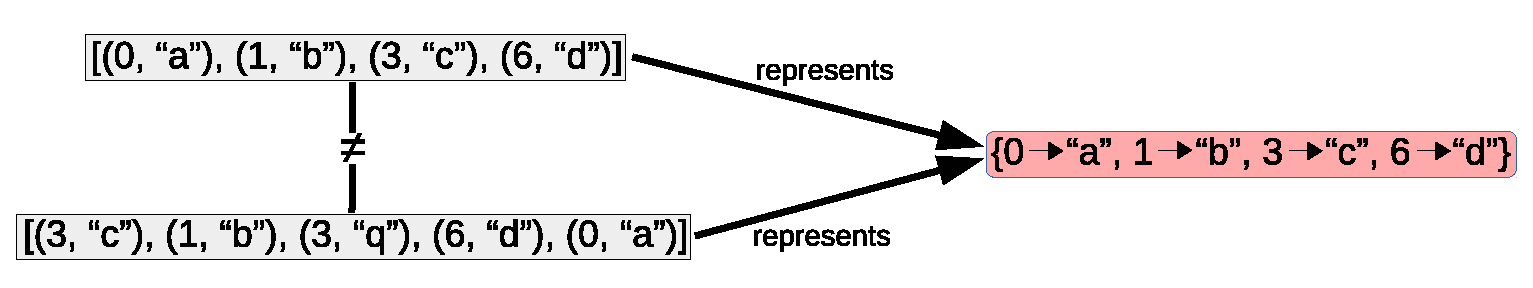
\includegraphics{figs/unequal.eps}};
    \end{tikzpicture}
    \caption{Same semantic mapping represented by unequal {\SAL}s}
    \label{fig:uneq}
  \end{figure}
Developing proofs is challenging, so any stumbling block, such as the inability to use a built-in equality
primitive to establish semantic equivalence of two objects, or the awkwardness of packaging
proof terms with data (noting the difficulties that arise from proof relevance), can cause exorbitant
increases in verbosity, time, effort, and accidental complexity. Since performance is often not a concern,
we have an opportunity to reassess the core criteria by which data structures are judged. Chiefly, these
new criteria will focus on alleviating or eliminating difficulties that crop up in the development of
proofs. In the \nameref{sec:Problem} section, we discuss several of these properties and argue for their
conceptual and practical importance.

The \cal~ (\CAL) and \fpf~ (\FPF) solutions (as well as ours) are set-like - i.e. they are insensitive
to duplication and ordering of insertions. As such, semantically equivalent dicts are also equal according
to the built-in equality primitive\footnote{Finite partial functions require the additional postulate of
\emph{functional extensionality}, which can be postulated
at essentially no cost given that it's been proven consistent with the constructive calculi underlying most
popular proof assistants (TODO SOURCE)}. However, \CAL~ and \FPF~ have other drawbacks.
If used as data, a \CAL~ must be refined with a proof of validity to ensure that it is ordered and deduped,
while equality is not decidable for {\FPF}s. In the \nameref{sec:Problem} section we discuss the difficulties
that arise from these drawbacks.

Our solution, which we dub {\dd}s, addresses the aforementioned problems by using a delta to
encode a key relative to its predecessor; instead of storing the key's literal value, we store the difference
from the previous key, minus 1 (details in section \nameref{sec:Mechanism}).
\\
\begin{tabular}{ l l }
 \quad\quad Delta dict & [(1, "b"), (1, "c"), (2, "d")]
\end{tabular}

Every list-of-pairs that type-checks is a valid \dd, and every unique \dd~ represents
a unique semantic mapping. So no proof term is needed to establish validity, there is a bijection between
\dd~ terms and finite maps, and if two {\dd}s are semantically equal, they must also be reflexively equal.

Naturally, {\dd}s have some drawbacks as well. The use of deltas requires that the key type not merely be
ordered but also possess a difference operation and a least element. Our definition and implementation uses
natural numbers for keys, and in section TODO we illustrate how to use bijections to the naturals as a way
of supporting strings, integers, or other key types that can be bijected to the naturals without great
difficulty. Although most types that are suitable for use as keys in the first place can be bijected to the
naturals, for some types defining this bijection may be too awkward or cumbersome, in which case {\dd}s may
be a poor choice.

Another drawback is that destruction and iteration of {\dd}s is substantially more
difficult than it is with the {\SAL}s or {\CAL}s, for which these operations are trivial
({\FPF}s cannot be properly destructed at all). As with the drawbacks of the other solutions, this one is
discussed further in the \nameref{sec:Problem} section.

TODO something something remaining sections, esp. Metatheory, Related Work, Conclusion, Discussion, or
whatever we wind up having.

\section{Problem}
\label{sec:Problem}
Data structures can possess or lack a wide range of properties that make them easier or harder to work with
when proving metatheory. Naturally, when possible, data structures should be chosen that posess those
properties which make the task at hand easier. Achieving this requires identifying the valuable properties,
what it is that makes them valuable, and finding or inventing data structures which possess those properties.
We hold that this is a broad topic of
research, which we illustrate in the particular context of choosing an implementation for a dictionary. In
this context, we identify, according to both conceptual and practical considerations, four important and
discriminating properties that a dictionary implementation may or may not possess:
TODO there's a good chance some of these properties have been named somewhere else. We should make sure we
don't try and coin terms for anything that's already been defined somewhere.
\newcommand{\SemTot}{\textit{Semantic Totality}}
\newcommand{\SemInj}{\textit{Semantic Injectivity}}
\newcommand{\EqDec}{\textit{Decidable Equality}}
\newcommand{\EzDstr}{\textit{Ease of Destruction}}
\begin{enumerate}
  \item \SemTot: Every term in the type is semantically valid, i.e. the mapping from
                 terms to their semantic meanings is total.
  \item \SemInj: Two unequal terms have different semantic meanings, i.e. the mapping
                 from terms to their semantic meanings is injective.
  \item \EqDec: Equality, in the sense primitive to the language at hand (particularly,
                reflexive equality rather than semantic equivalence) is decidable for the type.
  \item \EzDstr: The ease with which the data structure can be decomposed into its atomic
                 parts, to facilitate inspection or unrestricted non-additive manipulation.
\end{enumerate}

% TODO we may decide that the conceptual and practical benefits of decidable equality are so obvious or
% self-evident that we don't need any further discussion of that property

\subsection{Conceptual Importance}
\label{sec:Problem:concept}

In \autoref{sec:Problem:pract}, we illustrate practical problems and benefits under the particular context
of choosing an implementation for dictionaries. But first, it's worth exploring conceptual aspects that
apply to the general case. These conceptual aspects capture the spirit of practical considerations and
motivate the search for solutions that are not merely serviceable but elegant, moral, and insightful.

\subsubsection{\SemTot}
\label{sec:Problem:concept:SemTot}
TODO something something "making impossible states impossible", i think allusion to the right parts out of that
video will suffice to make the point here

\subsubsection{\SemInj}
\label{sec:Problem:concept:SemInj}
TODO something something it yields arbitrariness, which is not always wrong but which is unaesthetic and, when
avoidable, undesirable. It also allows for a semantic meaning to be represented by a concrete thing that is
needlessly verbose and complicated.

\subsubsection{\EqDec}
\label{sec:Problem:concept:EqDec}
The languages of proof assistants generally pride themselves on being total and constructive, on emphasizing
the knowable and demonstrable over the mysterious and hypothetical.

\subsubsection{\EzDstr}
\label{sec:Problem:concept:EzDstr}
TODO We need to clearly explain what we're talking about here, and clarify stuff like "facilitate inspection"
and "unrestricted non-additive manipulation". Aside from these clarifications, we won't say much else - in
this case the conceptual value largely boils down to the practical value.

\subsection{Practical Importance}
\label{sec:Problem:pract}
To illustrate practical problems and solutions, we present a hypothetical case study of a developer working to
prove evaluation metatheory using environment-based semantics. This case study closely resembles the actual process we went
through on a real project, the difficulties of which created the necessity of inventing {\dd}s. Of course,
because this case study involves a very particular situation, one which seems to be unusual (TODO sources?),
the problems we run into and solutions we suggest may not generalize. Accordingly, we use the case study to
present concrete illustrative examples, and follow each example with an argument of its applicability to more
general situations.

\newcommand{\eval}[3]{\ensuremath{{#1} \vdash {#2} \hspace{0.01in} \Rightarrow {#3}}}

At the outset, we have an evaluation judgment \eval{E}{e}{r}~ which takes an environment $E$ and an expression $e$
and "produces" a result $r$.
%Many mechanizations use substitution rather than environments, but (TODO source)
%explains why environment-based semantics are sometimes preferable. More generally, environments are only one use
%case for dictionaries, which are a very general purpose data structure that is likely to be used for a wide
%variety of other purposes.
$E$ is a finite map from variable names in scope to the results that are bound to
those variables. The question is "What data structure do we use to implement $E$?". The simple answer is a \sal,
and as long as we don't run into any problems on account of \SAL's lack of certain useful properties, the simple
answer is best.

But if we consider it important to prove the \emph{structural properties} \emph{contraction}
and \emph{exchange} (see \autoref{fig:con-exch}), we do run into a problem. These properties correspond,
respectively, to the irrelevance of duplication and reordering in the environment with regard to the judgment's
conclusions. The rule for lambda evaluation states that \mbox{\eval{E}{\lambda x . e}{[E]\lambda x . e}}, the result
being a closure over $E$. Using {\SAL}s, \mbox{\eval{E, (x, a), (x, b)}{\lambda x . e}{[E, (x, a), (x, b)]\lambda x . e}}
while \mbox{\eval{E, (x, b)}{\lambda x . e}{[E, (x, b)]\lambda x . e}}; $[E, (x, a), (x, b)]\lambda x . e \ne
[E, (x, b)]\lambda x . e$, so \emph{contraction} is violated. \emph{Exchange} is violated similarly. Many mechanizations
do not aim to prove \emph{contraction} and \emph{exchange} (TODO sources?), which makes our scenario somewhat
particular - however, they are two of the defining properties of structural logics, and as such are of critical
importance in many general cases (TODO source). Furthermore, inability to prove these theorems could be a red flag
of a bug in the judgment, so proving them has practical value, even if the judgment doesn't need to be strictly
structural.

%  \begin{figure}[H]
%    $
%    \inferrule*
%      {\eval{\lambda x . e}{}
%      {E, (x, b) \vdash T}
%    $
%    \caption{Evaluation rule for lambdas}
%    \label{fig:eval-lam}
%  \end{figure}

To address this problem, we need a data structure that possesses \SemInj. Since the semantics of dictionaries are
insensitive to duplication or ordering of insertions, the data structure must be likewise insensitive, so
that the language's equality primitive has the same meaning as semantic equality, and thus
\mbox{$E, (x, a), (x, b) = E, (x, b)$}. Note that proving \SemInj~ not only makes it possible to prove
\emph{contraction} and \emph{exchange}, but gives us these \emph{structural properties} essentially "for free".

  \begin{figure}[H]
    $
    \inferrule*[lab=\textbf{\large Contraction}]
      {\eval{E, (x, a), (x, b)}{e}{r}}
      {\eval{E, (x, b)}{e}{r}}
    $
    \quad\quad\quad\quad
    $
    \inferrule*[lab=\textbf{\large Exchange}]
      {\eval{E, (x, a), (y, b)}{e}{r} \\ x \ne y}
      {\eval{E, (y, b), (x, a)}{e}{r}}
    $
    \\\hfill\\\quad\quad
    $
      D, (x, a), (x, b) = D, (x, b)
    $
    \quad\quad
    $
      x \ne y \rightarrow D, (x, a), (y, b) = D, (y, b), (x, a)
    $
    \caption{Contraction and exchange theorems for \emph{eval}, as well as analogs for dictionary data structures that possess \SemInj (TODO source for contraction and exchange)}
    \label{fig:con-exch}
  \end{figure}

\newcommand{\refine}[2]{\ensuremath{{#1}\{\text{#2}\}}}

This problem can be addressed by switching from {\SAL}s to {\cal}s or {\fpf}s, because the latter two possess
\SemInj. Let's assume for the sake of discussion that we go with {\CAL}s. We run into another problem - {\CAL}s
do not possess \SemTot, because an arbitrary association list that type-checks may not be a valid \CAL.
An invalid association list can still be used in the same way a \SAL~ would, but we lose the
\SemInj~ property. Thus, wherever the \CAL~ goes, it must be refined with a proof of its validity. The ability
to refine ordinary types with proofs of validity is one of the most interesting and useful benefits of
dependently-typed languages, and this power should be appreciated. However, refining with proof terms can
come at a practical cost, so even in dependently-typed languages, there is high value in avoiding refinements
whenever possible (or at least whenever profitable). The practical cost of refinements is that proof terms
don't possess the properties \SemInj~ or \EqDec: due to \emph{proof relevance} (TODO source), two proofs of
the same property may be unequal, and due to the fact that proof terms may contain functions, the equality of
proof terms is not even decidable in the general case. With {\CAL}s, \mbox{$E, (x, a), (x, b) = E, (x, b)$},
but with refinements such as \refine{E}{proof\_of\_validity},
\mbox{$[\refine{(E, (x, a), (x, b))}{proof1}]\lambda x . e \ne [\refine{(E, (x, b))}{proof2}]\lambda x . e$},
so \emph{contraction} is once again violated. Perhaps we can work around this problem by moving the proof term
outside of the closure, to get \mbox{\refine{([E, (x, a), (x, b)]\lambda x . e)}{proof1}}, then defining a
special notion of equality for evaluation results, that treats closures specially by erasing the proof term
before checking equality with the built-in primitive, then definining \emph{contraction} and \emph{exchange}
in terms of this special notion of equality. However, this is all very cumbersome. We are no longer able to
use primitive equality when working with results, our special notion of equality should be decidable, but
not trivially so, and whenever we make any "modification" to an environment we must use theorems
to appropriately update the proof term and then repackage the new proof term with the new environment.
These sorts of pain points can crop up in any case where a refined object is being used as data, or must be
tested for equality with another refined object. Thus \SemTot, which obviates the need for refinement, has
a lot of practical value in many general cases.

{\FPF}s, sans refinement, do not technically satisfy \SemTot, because a type-correct function may not
actually be finite. However, since we can't iterate, destruct, or query the size of {\FPF}s, the code
that works with dictionaries doesn't actually need to ensure that those dictionaries are finite. Lookup
and insertion will work just the same on finite and infinite partial functions, so there's generally no
practical need to refine them with proofs of finititude. Thus we can avoid the problems of validity refinement
by switching from {\CAL}s to {\FPF}s. But doing so creates new problems, since unlike the association lists,
{\FPF}s don't possess \EqDec. We can prove that
\mbox{$[E, (x, a), (x, b))]\lambda x . e = [E, (x, b)]\lambda x . e$}, and thus prove \emph{contraction} and
\emph{exchange}, but there's no way to determine whether two arbitrary results are equal or unequal.
The ability to decide equality has very general utility; in our particular case, we had an
\mbox{$\texttt{assert}~ e_1 = e_2$} form which would evaluate $e_1$ and $e_2$ and then check if the results
were equal, naturally requiring that equality of results be decidable. Additionally, as aforementioned,
it's not possible to iterate, destruct, or query the size of {\FPF}s, a critical limitation if there's
ever a need to inspect the environment or delete a mapping from it.

At this point it was necessary to invent a dictionary data structure that had all three critical properties:
\SemTot, \SemInj, and \EqDec. \EqDec~ ruled out function-based techniques, \SemInj~ required canonical
ordering and deduplication, and \SemTot~ meant that the canonical order and deduplication had to come from
how the data was interpreted rather than how it was organized. These requirements essentially defined the
mechanism of {\dd}s. Of course, the non-literal way in which the data is interpreted means that it is not
safe for client code to work with the raw data directly, rather all interaction with the data must be
encapsulated in library functions. Unfortunately, this includes \emph{destruction}; an interaction which
normally goes through the very natural, elegant, and well-supported mechanism of pattern matching is now
only available through a library theorem:

\texttt{destruct-dd : (A : Type) (D : dd A) $\rightarrow \\
\phantom{xxxxxxxxxxxxxxxx} D = \emptyset \quad \lor \\
\phantom{xxxxxxxxxxxxxxxx} \exists~(n, a, D')~\left\{~ D = D' , (n, a) \quad \land \quad n \notin D' ~\right\}$}

Just as a list can be destructed with a case expression whose first branch matches nil and whose second branch
decomposes the list into a single item (particularly the head) and the remainder of the list, a \dd~ can be
destructed by matching the result of \texttt{destruct-dd} with a case expression whose left branch handles the
nil dictionary and whose right branch is provided a single item from the dictionary (the mapping $(n, a)$)
and the remainder of the dictionary ($D'$), as well as a proof that $D'$ really is $D$ minus the $(n, a)$
mapping.

This function achieves the same purpose as typical pattern matching (albeit more awkwardly), but because it
doesn't harness the primitive notions of pattern matching and structure, it doesn't establish structural
decrease on the dictionary object, which may break out-of-the-box structural recursion in the likely case
of recursion on $D'$. To enable manual establishment of structural recursion, via an extra parameter that
explicitly tracks the dictionary length, we provide another theorem:

\texttt{dd-extend-length : (A : Type) (D : dd A) (n : Nat) (a : A) $\rightarrow \\
\phantom{xxxxxxxxxxxxxxxxxxxxx} n \notin D \rightarrow \\
\phantom{xxxxxxxxxxxxxxxxxxxxx} |D, (n, a)| = 1 + |D|$}

Although possible, manually establishing termination is painful, especially given that it's not necessary
for {\SAL}s or {\CAL}s. Thus {\dd}s fail at \EzDstr, although they are still better than {\FPF}s in this
regard, seeing as it's not only hard but impossible to destruct {\FPF}s. Is it possible to have a data
structure that possesses all four properties? Not likely - as mentioned above, \SemTot~ essentially
necessitates that the data in the data structure be interpreted in a non-literal way, which in turn
makes it dangerous for client code to mess with the raw data. As such, we believe we've uncovered an
inherent trade-off between desirable properties. In our case, where \EqDec~ of results is critical,
and the need to destruct dictionaries is occasional but rare, {\dd}s seem to be a clear winner over
{\CAL}s ({\SAL}s and {\FPF}s are unviable for our requirements), but in cases where dictionaries are
not used as data
(e.g. as a subcomponent of a closure) or at least not data that needs to be tested with equality, and
where dictionaries sometimes need to be inspected or destructed, {\CAL}s may be a preferable.

\begin{figure}[H]
  \begin{tabular}{ l | c | c | c | c || c | c}
            & Sem. Total & Sem. Inj. & Dec. eq. & Destr.  & Simple & Key type requirement
   \\\hline
   \sal     & Yes        & No        & Yes      & Trivial & +1     & Decidable equality
   \\\hline
   \cal     & No         & Yes       & Yes      & Trivial & 0      & Orderable
   \\\hline
   \fpf     & No(TODO)   & Yes       & No       & No      & 0      & Decidable equality
   \\\hline
   \dd      & Yes        & Yes       & Yes      & Hard    & -1     & Bijects to naturals
  \end{tabular}
  \caption{Summary of the various data structures and which properties they possess}
  \label{fig:prop-summary}
\end{figure}

%Finally, because they guarantee the \emph{structural properties} \emph{contraction} and
%\emph{exchange}, {\dd}s are inherently inappropriate for substructural logics/judgments that reject one or
%both of those properties. In these cases, the naive solution's sensitivity to duplication and/or ordering is
%a feature, not a bug, and that solution becomes not only the natural solution but the morally correct one.
%Future work could explore the possibility of data structures that uphold one of these properties but not the
%other.

\section{Mechanism}
\label{sec:Mechanism}
List-of-pairs with ordered, "delta-encoded" keys;
instead of storing the raw keys, we store
the difference from the previous key, minus 1
\begin{figure}[H]
  \centering
  \begin{tikzpicture}[nodes = {align = left}]
    \node [scale=.45]
    {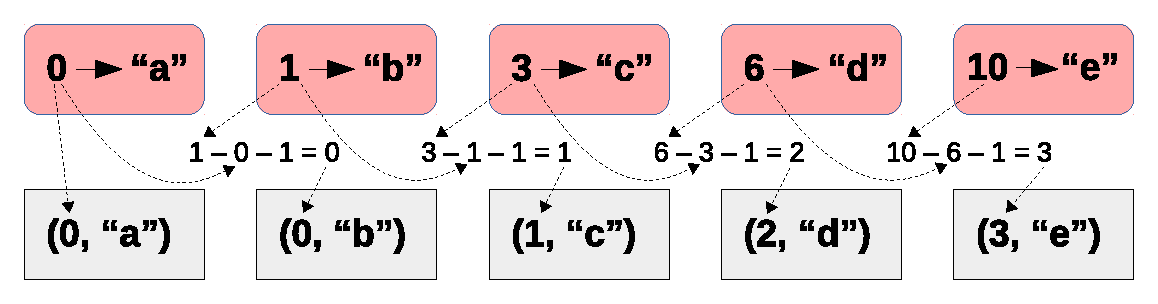
\includegraphics{figs/mech-1.eps}};
  \end{tikzpicture}
  \caption{How do we represent the mapping $\mapP$ as a \dd?}
  \label{fig:mech1}
\end{figure}
\begin{figure}[H]
  \centering
  \begin{tikzpicture}[nodes = {align = left}]
    \node [scale=.45]
    {\includegraphics{figs/find-6.eps}};
  \end{tikzpicture}
  \caption{How do we find key $6$ in the \dd?}
  \label{fig:find-6}
\end{figure}

TODO

\section{Metatheory}
\label{sec:Metatheory}
TODO

%\section{Evaluation}
%\label{sec:Evaluation}
% TODO delete? or keep?

\section{References}
\label{sec:References}
TODO TODO TODO - REFERENCES
\\
the second answer on this stack overflow suggests the finite partial function approach:
\\
https://stackoverflow.com/questions/47362451/creating-a-dictionary-map-in-coq
\\
oh hey appears that this is in software foundations too
\\
https://6826.csail.mit.edu/2019/lf/Maps.html
\\
Coq has list-based maps that retain sorted order, but not every list data is a valid mapping
\\
https://coq.inria.fr/library/Coq.FSets.FMapList.html
\\
Coq also has FMapPositive, which is a tree based on the binary representation
\\
This one seems to attach a canonicity proof to an ordinary list:
\\
http://www.cs.bc.edu/~tassarot/papers/iris-refinement/coqdoc/iris.prelude.natmap.html
\\
something something explicit substitutions, Abadi et al. POPL 1990.

\clearpage
%\bibliography{references,all.short}
\bibliography{references}

% \clearpage
% \appendix
% \input{implementation-appendix}

\end{document}
